% "{'classe':('PSI'),'chapitre':'dyn_pfd_co','type':('application'),'titre':'Banc d\\'essai vibrant', 'source':'Pôle Chateaubriand -- Joliot Curie','comp':('C1-05','C2-09'),'corrige':True}"
%\setchapterimage{bandeau}
\chapter*{Application \arabic{cptApplication} \\ 
Chaîne ouverte -- Banc d'essai vibrant \ifnormal $\star$ \else \fi \ifdifficile $\star\star$ \else \fi \iftdifficile $\star\star\star$ \else \fi
-- \ifprof Corrigé \else Sujet \fi}
\addcontentsline{toc}{section}{Application \arabic{cptApplication} : 
Chaîne ouverte -- Banc d'essai vibrant \ifnormal $\star$ \else \fi \ifdifficile $\star\star$ \else \fi \iftdifficile $\star\star\star$ \else \fi
-- \ifprof Corrigé \else Sujet \fi}

\iflivret \stepcounter{cptApplication} \else
\ifprof  \stepcounter{cptApplication} \else \fi
\fi

\setcounter{question}{0}
\marginnote{Pôle Chateaubriand -- Joliot Curie}
\marginnote{\xpComp{DYN}{05}}
%
%\marginnote[1cm]{
%\UPSTIcompetence[2]{C1-05}
%\UPSTIcompetence[2]{C2-09}
%}
\begin{marginfigure}
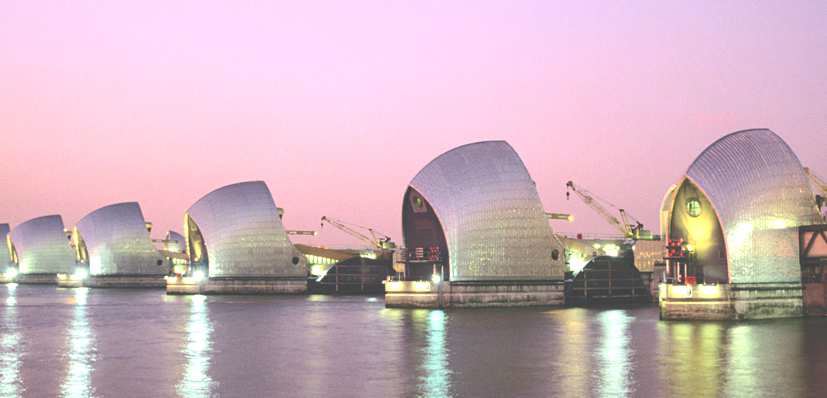
\includegraphics[width=\linewidth]{fig_00}
\end{marginfigure}


\subsection*{Présentation}
Les vibrations se retrouvent dans tous les systèmes et nuisent à leur durée de vie. On s’intéresse à un banc d’essai permettant d’étudier les conséquences de ces vibrations sur l’usure et la fatigue des pièces mécaniques.
La figure ci-après représente un modèle cinématique du dispositif étudié. Une modélisation plane a été retenue.
Le bâti vibrant est modélisé par un solide $S_1$, de masse $m_1$ en liaison glissière parfaite avec un support $S_0$, fixe par rapport à un repère $\mathcal{R}_0$ supposé galiléen.

Le solide $S_1$ est rappelé par un ressort de longueur libre $l_0$ et de raideur $k$.
Une masse ponctuelle $m_2$ excentrée, placée en $P$, tourne sur un rayon $r$ et est entraînée à vitesse constante $\Omega$. Elle modélise le 
balourd du rotor d’un moteur $S_2$.

Un pendule simple de longueur $L$, porte à son extrémité $D$ une masse concentrée $m_3$, l’ensemble constitue le solide $S_3$, en liaison pivot parfaite d’axe $\axe{C}{z_0}$ avec $S_1$.

Les masses autres que $m_1$, $m_2$ et $m_3$ sont négligées.



\begin{marginfigure}
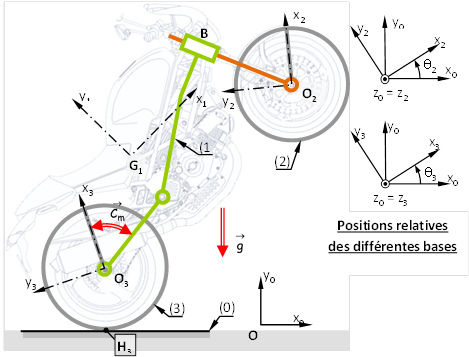
\includegraphics[width=\linewidth]{fig_01}
\end{marginfigure}

\begin{obj}
Déterminer les conditions géométriques permettant de supprimer les vibrations.
\end{obj}

\question{Réaliser le graphe d'analyse du système.}
\ifprof
\begin{corrige}
\end{corrige}
\else
\fi


\question{Préciser les théorèmes à utiliser permettant de déterminer deux équations différentielles liant $x$, $\theta$ et leurs dérivées et les paramètres cinétiques et cinématiques utiles.}
\ifprof
\begin{corrige}
\end{corrige}
\else
\fi


\question{Déterminer ces deux équations.}
\ifprof
\begin{corrige}
\end{corrige}
\else
\fi
On souhaite supprimer les vibrations du bâti vibrant. On recherche alors une solution du système d’équations différentielles
déterminé précédemment autour de la position d’équilibre $\left(x_0,\theta_0\right)=(0,0)$ en supposant que $x$, $\theta$, $\dot{x}$, $\dot{\theta}$ sont des petites variations
de position ou de vitesse autour de cette position d’équilibre.


\question{Proposer une linéarisation, à l’ordre 1, des deux équations différentielles précédentes.}
\ifprof
\begin{corrige}
\end{corrige}
\else
\fi

On s’intéresse uniquement au régime d’oscillations forcées. On cherche donc des solutions de la forme $x(t)=A\cos\left( \Omega t \right)$ et $\theta(t)=B\cos\left( \Omega t \right)$.


\question{Déterminer le système d’équations permettant de calculer $A$ et $B$.}
\ifprof
\begin{corrige}
\end{corrige}
\else
\fi



\question{Indiquer la condition que doit vérifier la longueur $L$ afin d’assurer $x(t) = 0$ en régime forcé.}
\ifprof
\begin{corrige}
\end{corrige}
\else
\fi




\ifcolle
\else

\footnotesize
%\marginnote[-4cm]{
\begin{solution}
\begin{enumerate}
\item $\left( m_1 + m_2 + m_3\right) \ddot{x} + kx + m_3 L\ddot{\theta} \cos \theta - m_3 L\dot{\theta}^2 \sin \theta = m_2 r \Omega^2 \cos \left( \Omega t \right)$ et $\ddot{x}\cos\theta+L\ddot{\theta}+g\sin\theta=0$.
\item $\left( m_1 + m_2 + m_3\right) \ddot{x} + kx + m_3 L\ddot{\theta}= m_2 r \Omega^2 \cos \left( \Omega t \right)$ et $\ddot{x}+L\ddot{\theta}+g\theta=0$.
\item $A=\dfrac{m_2 r \Omega^2 \left( -L\Omega^2 + g\right)}{\left[-\left( m_1 + m_2 + m_3\right)\Omega^2 +k\right]\left( -L\Omega^2 +g\right)-m_3L\Omega^4}$ et 
$B=\dfrac{m_2 r \Omega^2 }{\left[-\left( m_1 + m_2 + m_3\right)\Omega^2 +k\right]\left( -L\Omega^2 +g\right)-m_3L\Omega^4}$.
\item $L=\dfrac{g}{\Omega^2}$.
\end{enumerate}
\end{solution}
%}
\normalsize
\fi


\ifprof
\else
\begin{marginfigure}
\centering

\includegraphics[width=3cm]{Cy_04_03_PFD_CO_App_02_BancVib_qr}
\end{marginfigure}
\fi

\ifprof
\begin{center}
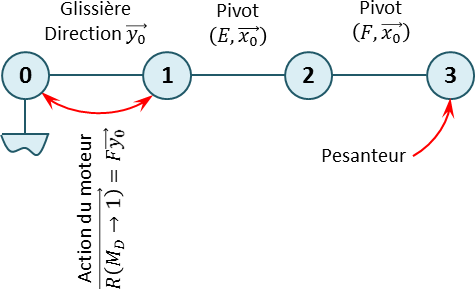
\includegraphics[width=.8\linewidth]{cor_01}
\end{center}

\begin{center}
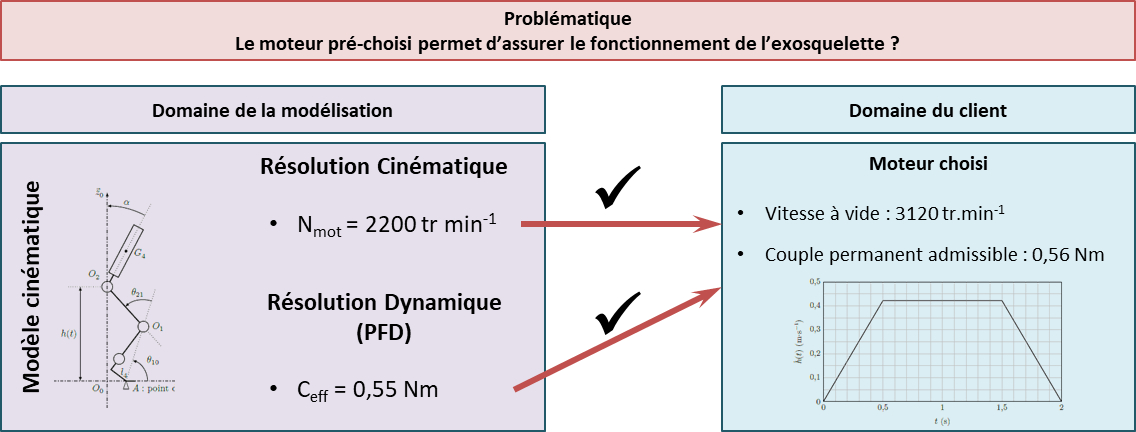
\includegraphics[width=\linewidth]{cor_02}
\end{center}

\begin{center}
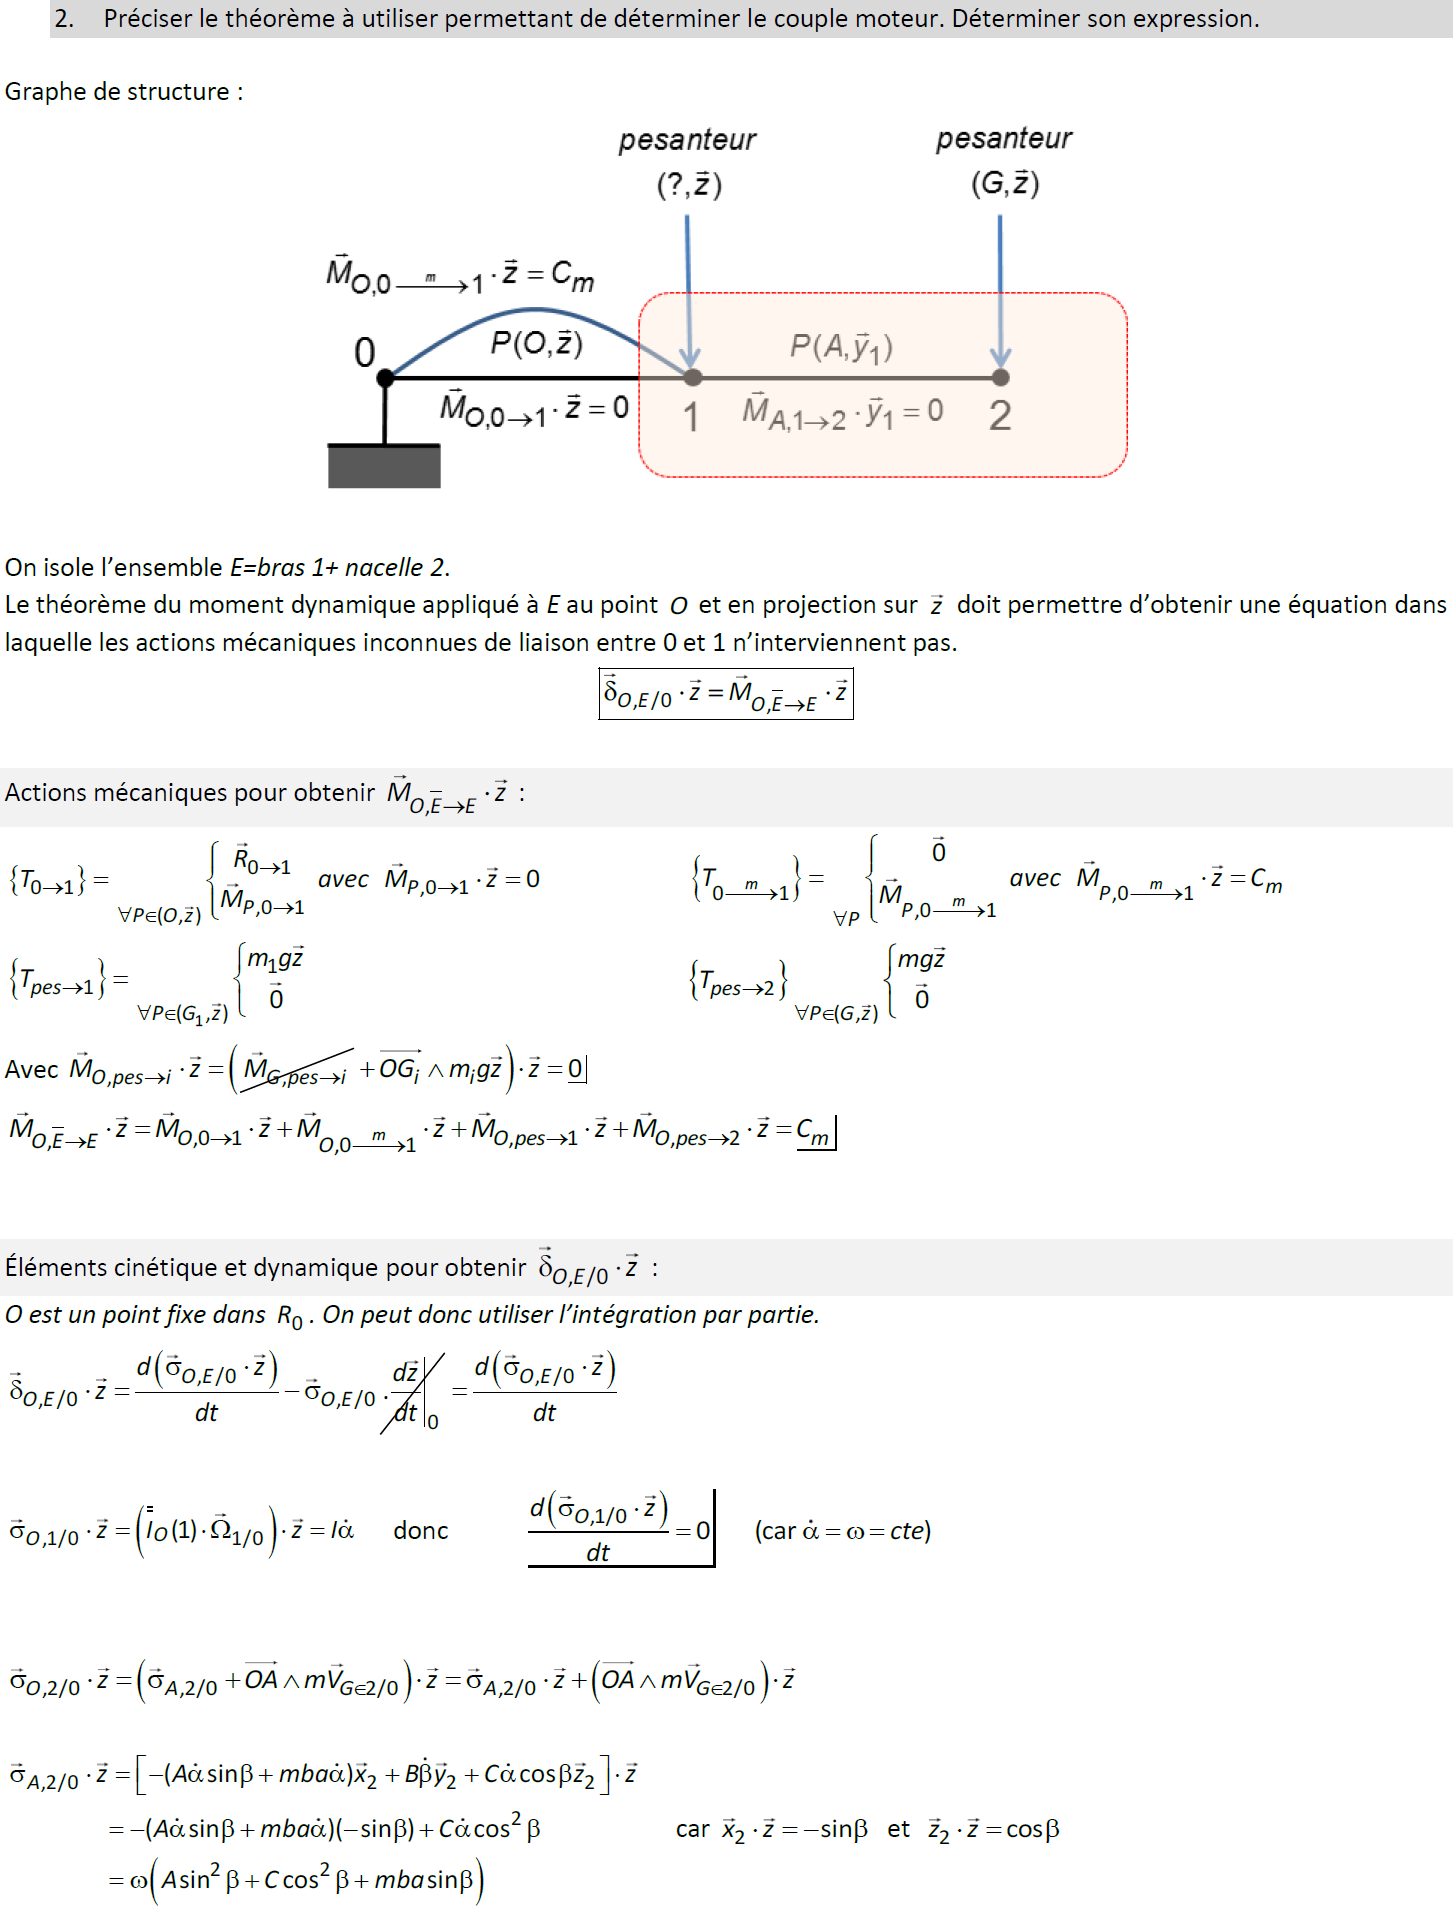
\includegraphics[width=\linewidth]{cor_03}
\end{center}
\else
\fi